\documentclass[10pt]{beamer}

%%%
% PREAMBLE FOR THIS DOC 
%%%
%https://tex.stackexchange.com/questions/68821/is-it-possible-to-create-a-latex-preamble-header
\usepackage{/Users/miw267/Repos/latex_preamble/beamer_preamble}

\usetikzlibrary{matrix}

\usetikzlibrary{shapes.geometric}

\usepackage{pgfplots} % For drawing histograms
\usetikzlibrary{pgfplots.groupplots} % For grouping multiple plots


%%% TRY TO RESHOW TOC AT EACH SECTION START (with current section highlighted)
% Reference: https://tex.stackexchange.com/questions/280436/how-to-highlight-a-specific-section-in-beamer-toc
\newcommand\tocforsect[2]{%
  \begingroup
  \edef\safesection{\thesection}
  \setcounter{section}{#1}
  \tableofcontents[#2,currentsection]
  \setcounter{section}{\safesection}
  \endgroup
}


%%%% HERES HOW TO DO IT CORRECTLY
% FIRST IN .STY FILE, DO
%\usetheme[sectionpage=none]{metropolis}
% THEN AT EACH SECTION DO
%\begin{frame}{Outline}
%  \tableofcontents[currentsection]	
%\end{frame}



%\setbeamertemplate{navigation symbols}{}
%\setbeamertemplate{footline}[frame number]{}


%%%
% DOCUMENT
%%%

\begin{document}

%\maketitle

%% Title page frame
%\begin{frame}
%    \titlepage 
%\end{frame}



\title{10/16/2026: Recurrence}
\author{CSCI 246: Discrete Structures}
\date{Textbook reference: Sec 23, Scheinerman}

\begin{frame}
    \titlepage 
\end{frame}


\begin{frame}
%\small
\begin{mygreenbox}[title=Quiz Retake Pickup]
Quiz retakes are in the front of the room, grouped into four bins (A-G, H-L, M-R, S-Z) by last name. The midterms are upside down with your last name on the back. Come find yours before, during, or after class.  Only turn the quiz over if it's yours.
\end{mygreenbox} 
\vfill 
\begin{myredbox}[title=Announcements]
\begin{enumerate}
	\item If you answered the playlists problem on the midterm in terms of combinations rather than permutations, see me.
	\item Detail on induction step: we assume any $k$ 
	\textbf{greater than or equal to the base}, and then show the claim must hold for $k+1$.
\end{enumerate}
\end{myredbox} 
\vfill 
\begin{myyellowbox}[title=Today's Agenda]
\begin{itemize}
	\item Weekly quiz (20 mins)
	\item Mini lecture ($\approx$ 15 mins)
	\item Group exercises ($\approx$ 15 mins)
\end{itemize}
\end{myyellowbox}
\vfill 

\end{frame}


\begin{frame}[standout]
Mini-lecture on recurrence
\end{frame}


\begin{frame}{Tower of Hanoi}
In 1883, French mathematician \'{E}douard Lucas invented a puzzle, based on an old Indian legend, called the \textbf{Tower of Hanoi}.

   \begin{center}
 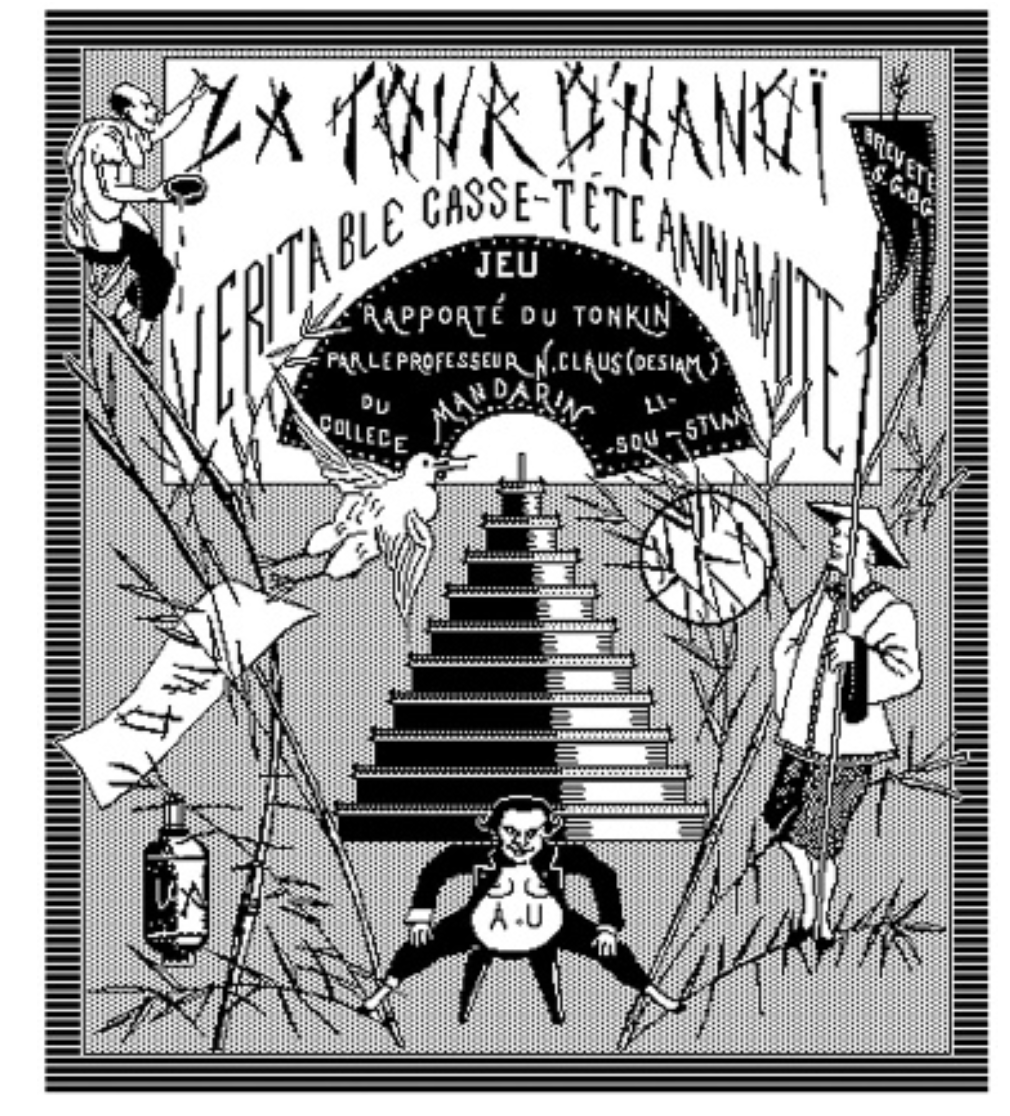
\includegraphics[width=0.4\textwidth]{images/tower_of_hanoi_cover}
   \end{center}
\vfill 
\vspace{-.2cm}
\colorbox{green!30}{\textbf{Prize.}} 
The puzzle offered 10,000 francs (about \$45,000 USD today) to anyone who could solve the puzzle with 64 disks. 

\vfill 
\pause 
\colorbox{red!30}{\textbf{Legend.}} According to the legend, when the puzzle is solved, the world will end.

\end{frame}




\begin{frame}{Tower of Hanoi}


   \begin{center}
 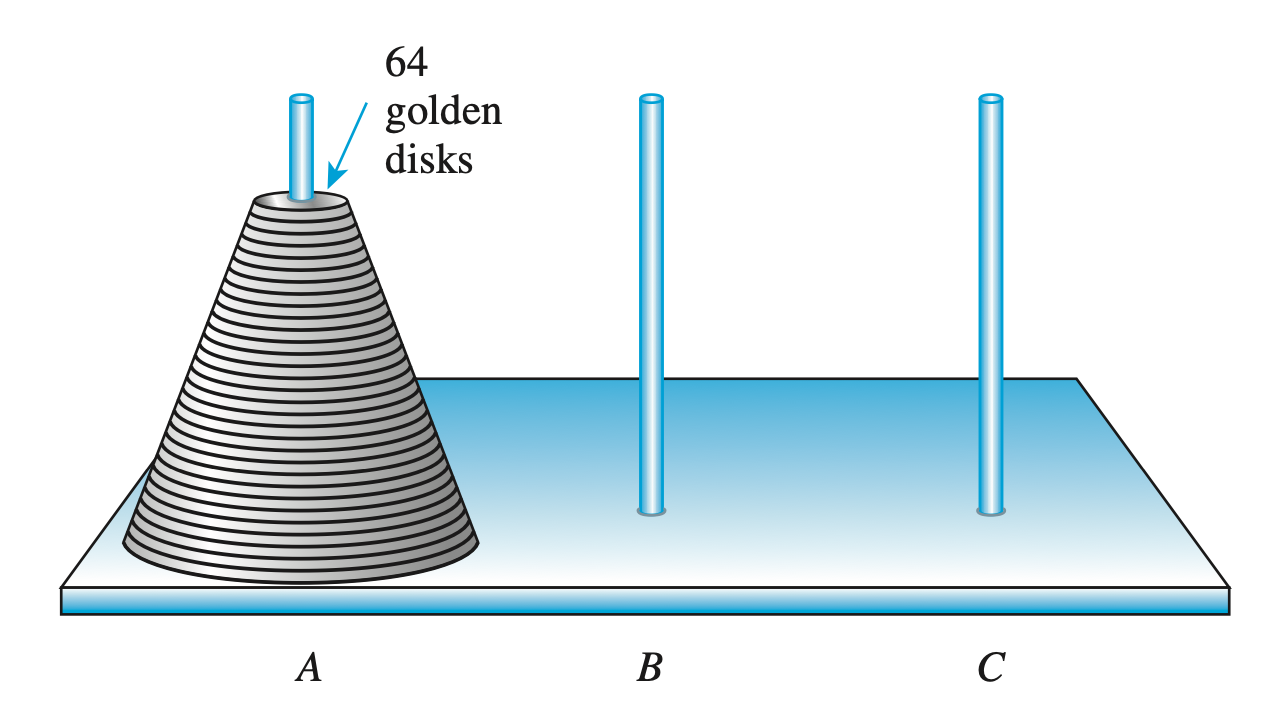
\includegraphics[width=0.7\textwidth]{images/tower_of_hanoi}
   \end{center}

\vfill 
\colorbox{red!30}{\textbf{Rules.}} 
\begin{itemize}
\item You must move all disks one by one from one pole to another.
\item You must never place a larger disk on top of a smaller one.	
\end{itemize}

\end{frame}
	
	
\begin{frame}{Tower of Hanoi: Solution As A Recursion}
    \centering

 \colorbox{green!30}{\textbf{Idea.}} Suppose you know the optimal solution for $k-1$ disks.  Then here's the optimal solution for $k$ disks.
 \vfill     
    \begin{minipage}{0.48\textwidth}
        \centering
        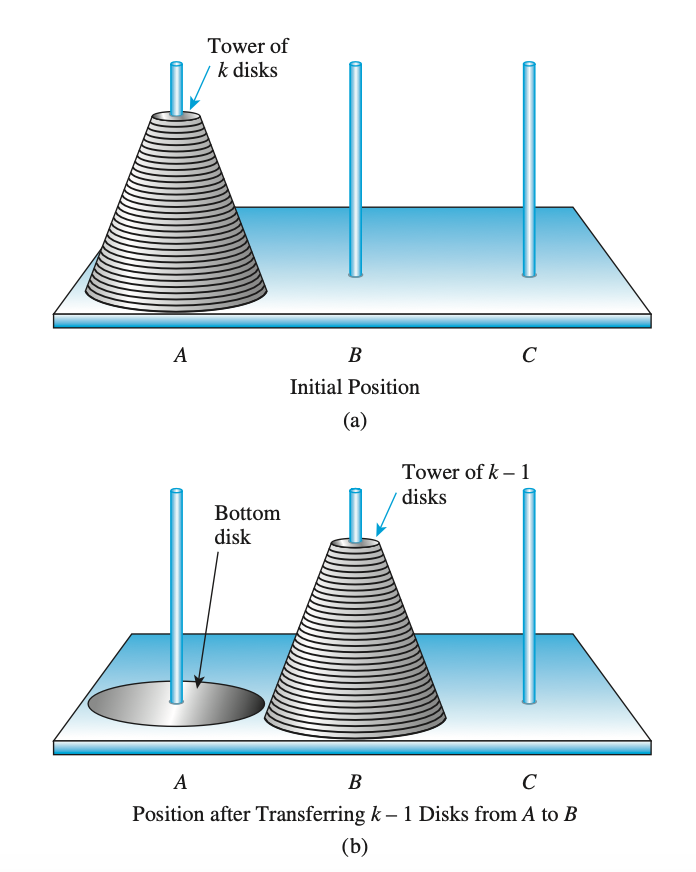
\includegraphics[width=\textwidth]{images/tower_of_hanoi_solution_1}
    \end{minipage}
    \hfill
    \begin{minipage}{0.48\textwidth}
        \centering
     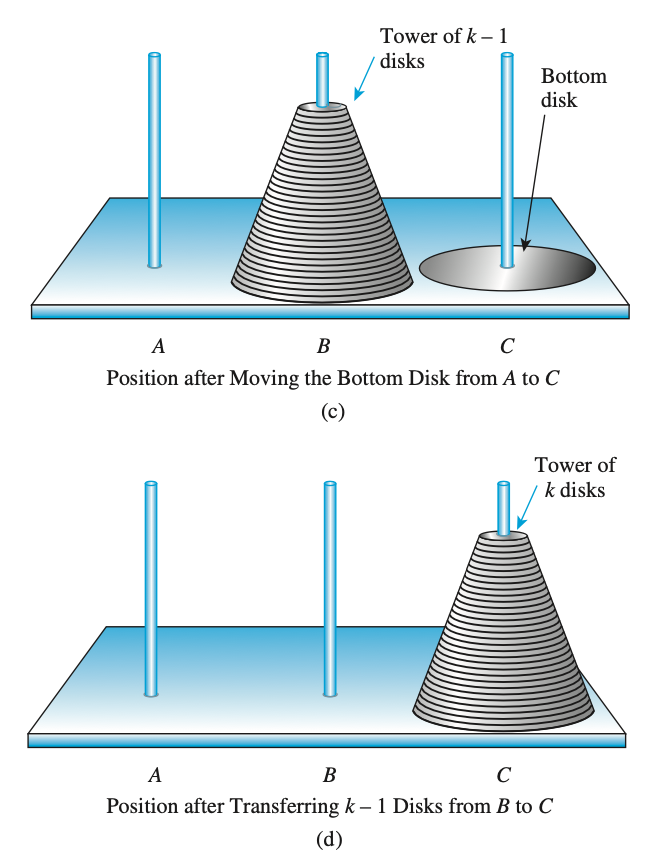
\includegraphics[width=\textwidth]{images/tower_of_hanoi_solution_2}
    \end{minipage}
\end{frame}
	
\begin{frame}{Tower of Hanoi: Solution As A Recursion}

\only<1->{Let $m_k$ be the minimum number of moves needed to transfer a tower of $k$ disks from one pole to another.}
\vfill 

\only<2-3>{\colorbox{yellow!30}{\textbf{Poll.}} Can you provide a recursive formula for $m_k$?}
\vfill 

\only<3>{\colorbox{green!30}{\textbf{Solution.}} 
From the last slide, we have
%
\begin{align*}
m_k &= m_{k-1} + 1 + m_{k-1} \\
	&= 2 m_{k-1} + 1
\end{align*}
}

\only<4->{\colorbox{yellow!30}{\textbf{Poll.}} We have derived a recursive formula for $m_k$ as \[m_k = 2 m_{k-1} + 1. \] 

So long would it take to solve the puzzle? 
}

\only<5->{\colorbox{green!30}{\textbf{Solution.}} Using the techniques from the textbook, we can derive the explicit formula
\[ m_k = 2^k - 1.\]}


\only<6>{(Note: This solution can be verified by induction!)}

\only<7>{\colorbox{yellow!30}{\textbf{Poll.}} What does this say about the prospects for winning the prize?}


\only<8->{Using this, we find  $m_{64} \approx 1.88 \times 10^{19}$.  In other words, if you work rapidly, and move one disk every second, the total number of time it would take to solve the puzzle with 64 disks is: \alert{584.5 billion years}! }
\end{frame}



\begin{frame}{Recursions are everywhere!}

\textbf{Some examples from textbooks:}

\begin{itemize}
  \item Fibonacci sequence (e.g., population growth)
  \item Compound interest
\end{itemize}

\begin{center}
\begin{minipage}{0.8\textwidth}
\centering
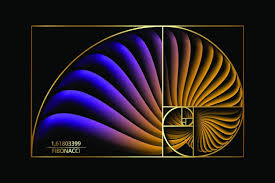
\includegraphics[height=2cm]{images/fibonacci.jpeg} \hspace{1em}
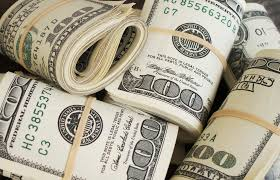
\includegraphics[height=2cm]{images/bank.jpeg}
\end{minipage}
\end{center}

\vfill
\textbf{Some examples from real-life software:}

\begin{itemize}
  \item Reinforcement learning (e.g., computer chess)
  \item Early cancer detection
\end{itemize}

\begin{center}
\begin{minipage}{0.8\textwidth}
\centering
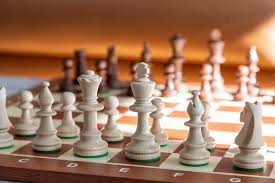
\includegraphics[height=2cm]{images/chess.jpeg} \hspace{1em}
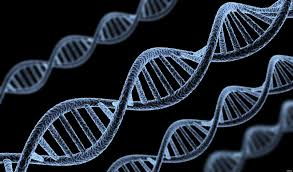
\includegraphics[height=2cm]{images/genes.jpeg}
\end{minipage}
\end{center}

\end{frame}


\begin{frame}[fragile]{Recursive programs are slow}
\footnotesize 
Consider the program to solve  $a_n = 3 a_{n-1} - 2 a_{n-2}$ with initial conditions $a_0=1, a_1=5$:
\begin{python}
def get_term(n):
    if (n < 0):
    	print("Illegal argument")
    elif (n==0):
    	return 1
    elif (n==1):
    	return 5
    else:
        return 3*get_term(n-1) - 2*get_term(n-2)
\end{python}
	
\pause \colorbox{yellow!30}{\textbf{Poll.}} How many times is this program called in order to calculate $a_n$?
\pause \vfill 

\colorbox{green!30}{\textbf{Solution.}} 
From the last line, the program is called
\[ b_n = b_{n-1} + b_{n-2} + 1\]
times to get term $a_n$.  The first few terms are 1,1,3,5,9,15,25.\\

\vfill \pause 
\vspace{.2cm}
\colorbox{red!30}{\textbf{Problem.}} This program is expensive to run! To get the 50-th term $a_{50}$, the program must be called $b_{50} \approx 40.7$ billion times!
 
\end{frame}



\begin{frame}[plain]
\begin{tikzpicture}[remember picture, overlay]
  % Background image, stretched to fill the whole slide
  \node[inner sep=0pt] at (current page.center)
    {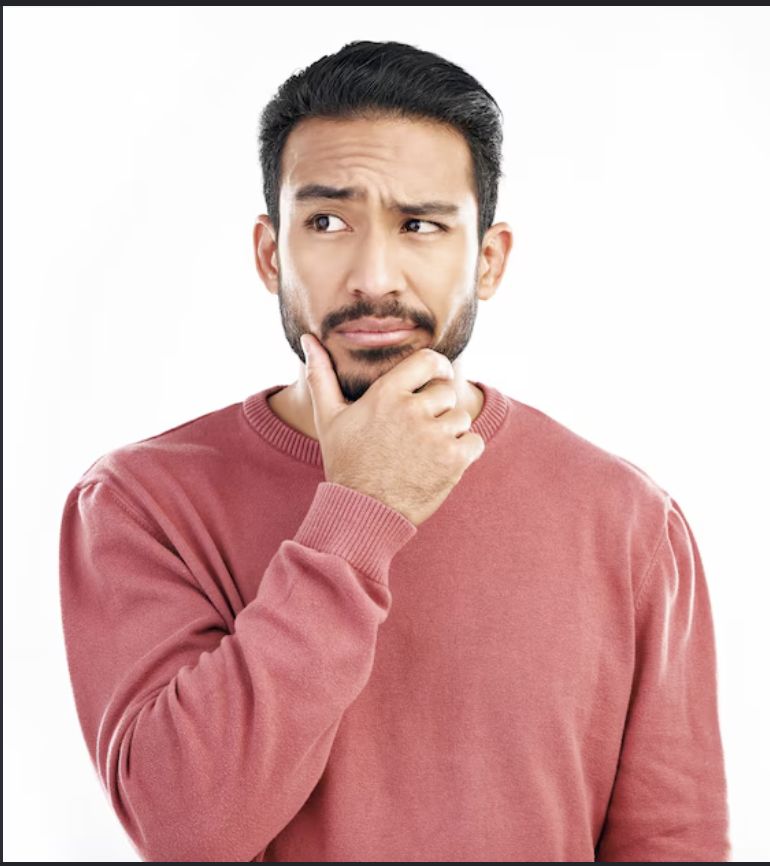
\includegraphics[width=\paperwidth, height=\paperheight]{images/thinking_face}};
  % Optional dark tint so the text stays readable on any photo
  \fill[black, opacity=0.35] (current page.south west) rectangle (current page.north east);
  % Large centered text
  \node[text=white, font=\Huge\bfseries, align=center, text width=0.85\paperwidth]
    at (current page.center) {Is there a better way to handle recursions?};
\end{tikzpicture}
\end{frame}

\begin{frame}{Three ways to represent sequences}

\colorbox{green!30}{\textbf{1. Writing the first few terms.}} E.g.: Consider the sequence $3,5,7,\hdots.$ \pause 
\vfill 
\colorbox{blue!30}{\textbf{Evaluation.}} \pause  
\includegraphics[width=0.05\textwidth]{images/sad}  \underline{Misunderstandings} can occur.  \pause The next sequence could be 9 (if we mean odd integers) or 11 (if we mean odd prime integers). \pause 
\vfill\vfill 
\colorbox{green!30}{\textbf{2. State a recurrence relation.}} \pause E.g. $a_n = 5 a_{n-1} + 3$ with initial condition $a_0=1$. \pause 
\vfill 
\colorbox{blue!30}{\textbf{Evaluation.}} \pause  
\includegraphics[width=0.05\textwidth]{images/neutral} More clear. However, the \underline{computation} to obtain the $n$-th term can be prohibitive. (See previous slides.) \pause 
\vfill\vfill 
\colorbox{green!30}{\textbf{3. Give an explicit formula for the $n$-th term.}} E.g.  
\[ a_n = \frac{7}{4} \cdot 5^n -\frac{3}{4}.\]
\vfill  
\colorbox{blue!30}{\textbf{Evaluation.}} 
\includegraphics[width=0.05\textwidth]{images/happy} \pause  This is the best situation to be in. Clear and quick.  The textbook gives techniques for obtaining these.
\end{frame}








\begin{frame}{Most important results from the textbook -- Part 1}

\begin{mygreenbox}[title=\text{Solving first-order recurrences (Props 23.1, 23.3)}]
All solutions to recurrence relation $a_n = s a_{n-1} + t$ have the form
\[
a_n = 
\begin{cases}
c_1 s^n + c_2, & \text{ if } s \neq 1 \\
a_0 + nt, & \text{ if } s = 1 \\
\end{cases}
\]
\end{mygreenbox}
\vfill 
\pause 

\only<2->{
\colorbox{blue!30}{\textbf{Remark.}} In the first group exercise, we'll apply this to solve the Tower of Hanoi problem!
}

\only<3->{
\begin{mygreenbox}[title=\text{Solving second-order recurrences (Thms 23.5, 23.9)}]
All solutions to recurrence relation $a_n = s_1 a_{n-1} + s_2 a_{n-2}$ have the form
\[
a_n = 
\begin{cases}
c_1 r_1^n + c_2r_2^n, & \text{ if } r_1 \neq r_2 \\
c_1 r^n + c_2 n r^n, & \text{ if } r_1 =  r_2 \defeq r \\
\end{cases}
\]
%
where $r_1, r_2$ are roots of $x^2 - s_1x - s_2 =0$.
\end{mygreenbox}
}

\end{frame}


%\begin{frame}{Recurrences are discrete-time differential equations}
%\footnotesize
%\begin{tabular}{@{}l l l@{}}
% & \textbf{Continuous time} (differential eq.) & \textbf{Discrete time} (recurrence) \\
%\textbf{1D} & $x'(t) = k\,x(t)$ \; $\Rightarrow$ \; $x(t) = x(0)\,e^{kt}$ & $a_n = s\,a_{n-1}$ \; $\Rightarrow$ \; $a_n = a_0\, s^n$ \\
%\textbf{2D} & $x'(t) = A\,x(t)$ \; $\Rightarrow$ \; $x(t) = e^{tA} x(0)$ & $x_n = M x_{n-1}$ \; $\Rightarrow$ \; $x_n = M^n x_0$
%\end{tabular}
%
%\vspace{.1cm}
%Below, $M = \begin{psmallmatrix} 0.8 & -0.4 \\ 0.4 & 0.8 \end{psmallmatrix} = e^{A}$, so the discrete solution is the continuous one \textbf{sampled at} $t = 0, 1, 2, \ldots$  Each coordinate of $x_n$ obeys $a_n = 1.6\, a_{n-1} - 0.8\, a_{n-2}$, whose roots $r = 0.8 \pm 0.4i$ are complex: hence the \textbf{spirals}.
%
%\begin{center}
%\transduration<2-24>{0.3}
%\foreach \f [count=\s] in {00,01,02,03,04,05,06,07,08,09,10,11,12,13,14,15,16,17,18,19,20,21,22,23,24}{%
%  \only<\s>{\includegraphics[width=0.82\textwidth]{images/vector_field/frame_\f.png}}%
%}
%\end{center}
%\end{frame}


\begin{frame}{Fun Note: Recurrences are discrete-time differential equations}
\footnotesize
\begin{tabular}{@{}l l l@{}}
 & \textbf{Continuous time} (differential eq.) & \textbf{Discrete time} (recurrence) \\
 & $x'(t) = k\,x(t)$ \; $\Rightarrow$ \; $x(t) = x(0)\,e^{kt}$ & $a_n = s\,a_{n-1}$ \; $\Rightarrow$ \; $a_n = a_0\, s^n$ \\
\end{tabular}

\vspace{.1cm}
Below, each coordinate of obeys $a_n = 1.6\, a_{n-1} - 0.8\, a_{n-2}$, which gives \textbf{spirals}.

\begin{center}
\transduration<2-24>{0.3}
\foreach \f [count=\s] in {00,01,02,03,04,05,06,07,08,09,10,11,12,13,14,15,16,17,18,19,20,21,22,23,24}{%
  \only<\s>{\includegraphics[width=0.82\textwidth]{images/vector_field/frame_\f.png}}%
}
\end{center}
\end{frame}


\begin{frame}{Most important results from the textbook -- Part 2}

Thm 23.17 shows how to find a polynomial expression to generate the first few terms of a sequence.

\vfill 
\begin{center}
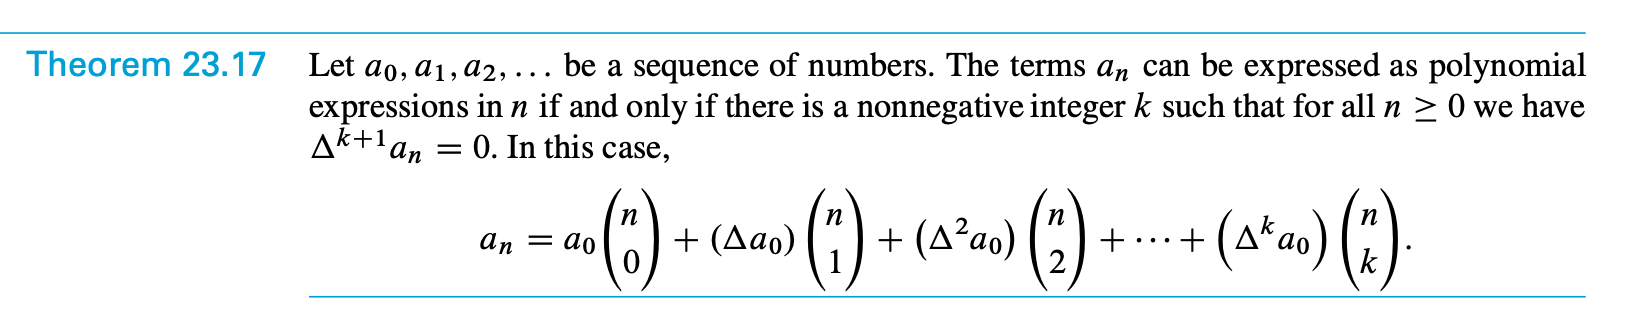
\includegraphics[width=\textwidth]{images/theorem.png}	
\end{center}
	
\end{frame}

\begin{frame}[standout]
Group exercises
\end{frame}


\end{document}
